\documentclass[../main.tex]{subfiles}
\begin{document}
\subsection{Determine}
This checklist is used to audit and verify the compliance of administrative acts (referred to as "determine") within a municipality. It ensures that each act meets the required legal and procedural standards by evaluating various key aspects:

\begin{itemize}
    \item \textbf{Authority and Competence:}
 Verifies whether the determination correctly identifies the competent authority or manager responsible for issuing the act, often established by a formal decree.
    \item \textbf{Document Structure:}
 Checks that the determination is properly organized, including sections such as the header, preamble, motivation, decision, and indications of the authorizing authority, deadlines for appeal, and references to the document's digital archive.
    \item \textbf{Legal References:}
 Ensures the document includes both general normative references (for example, references to overarching laws such as TUEL) and specific legal references (such as specific contract codes or internal regulations).
    \item \textbf{Inclusion of Activities:}
 Confirms that any activities mentioned in the determination are consistent with other planning documents (such as budgeting or program plans), and that timelines and project phases are clearly delineated.
    \item \textbf{Explicit Motivation:}
 Verifies that the act provides clear reasoning and justification, citing both factual premises and legal bases.
    \item \textbf{Responsibility and Delegation:}
 Checks for clarity on roles, such as the identification of the person responsible for the process or the delegation of duties, ensuring that responsibilities are properly assigned.
    \item \textbf{Preventive Measures:}
 Assesses whether the determination includes measures to prevent conflicts of interest, ensure transparency (such as publication requirements), and other specific protective steps related to performance objectives.
    \item \textbf{Privacy and Confidentiality:}
 Ensures that the act adheres to data protection and confidentiality regulations where applicable.
    \item \textbf{Timeliness:}
 Confirms that the act respects the required procedural timeframes and deadlines.
    \item \textbf{Additional Notes:}
 Allows for the identification of any further observations or critical issues, such as opportunities for simplification, digitalization, focus on specific priorities like equal opportunity or accessibility.
\end{itemize}
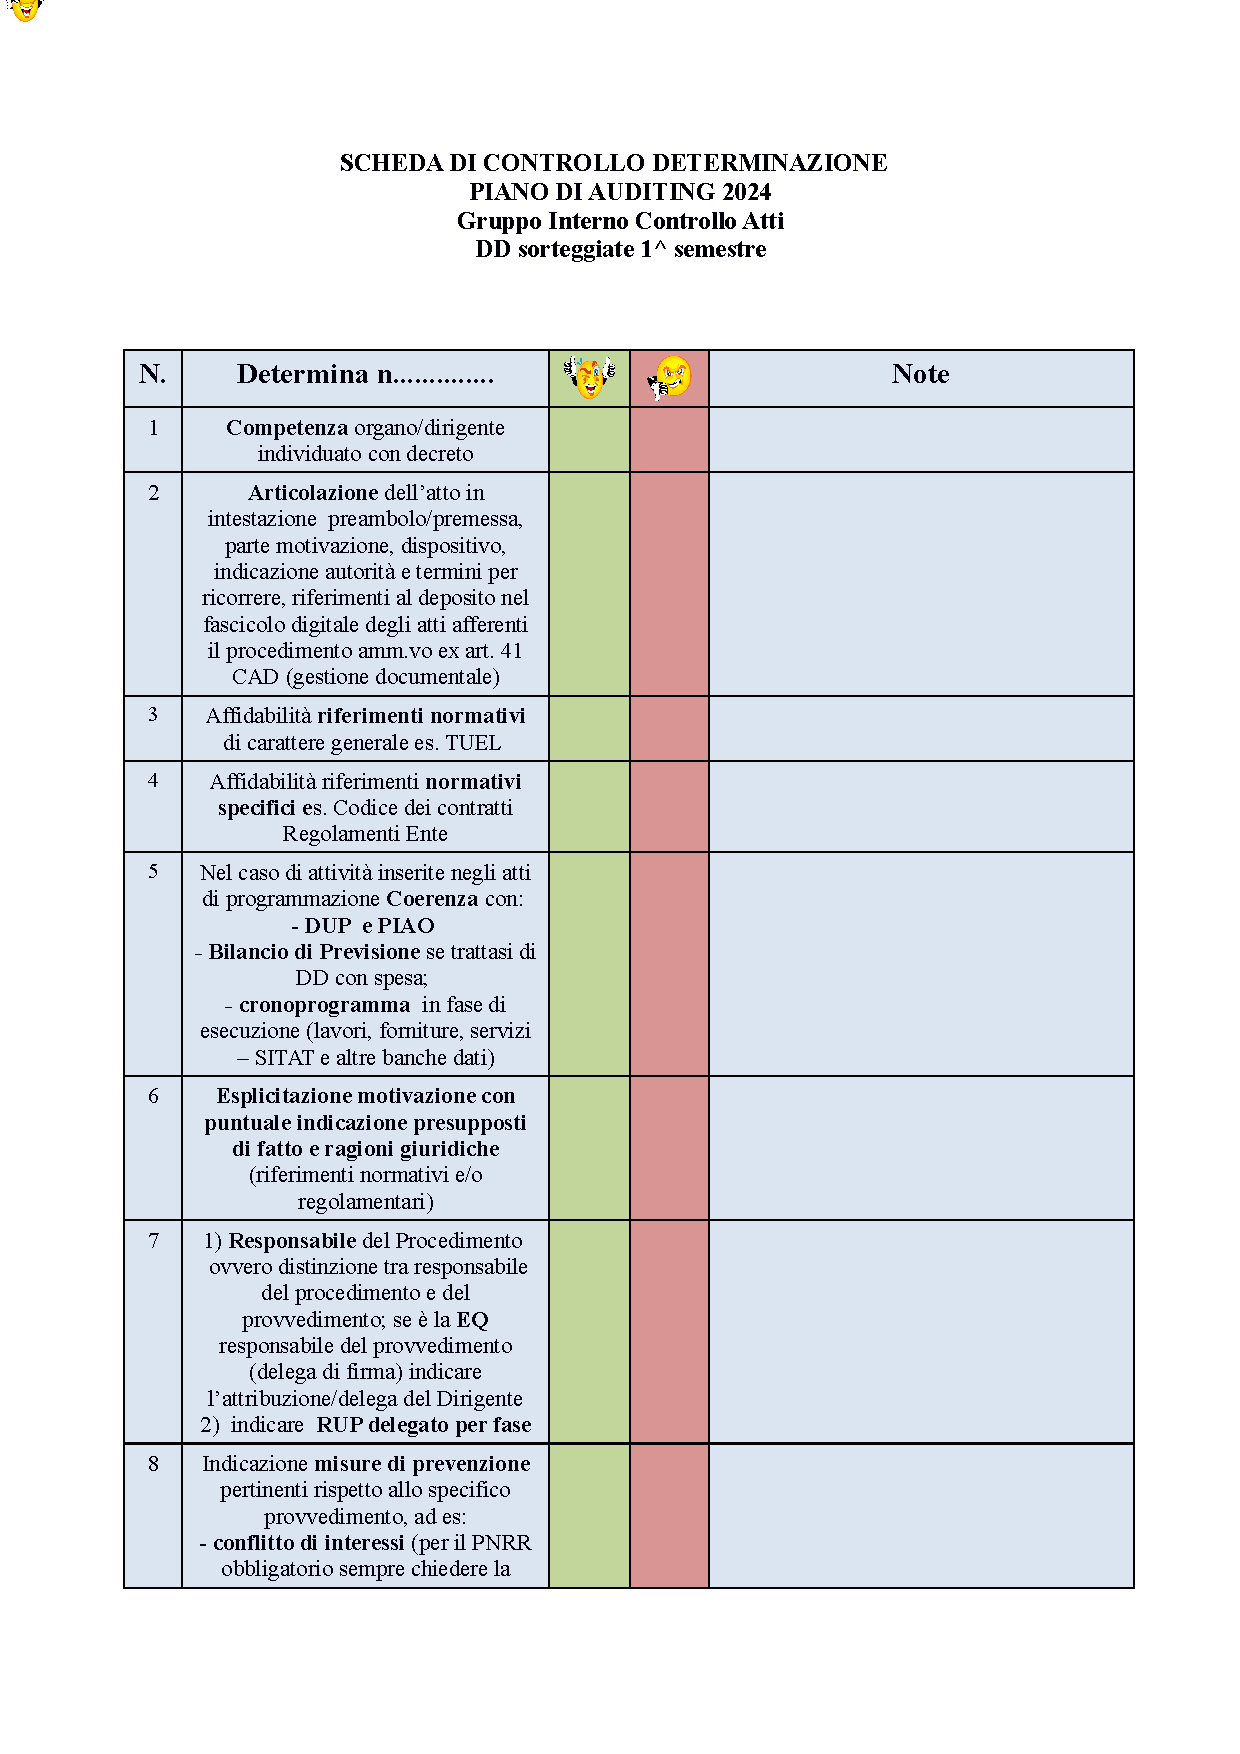
\includepdf[pages=-,scale=0.95,pagecommand={\section*{}}]{Checklists/Lucca/Determine}

\subsection{Contratti}
This checklist is tailored to the review of public contracts, focusing on verifying that contracts comply with administrative and legal standards, particularly those governing public procurement and contract management:

\textbf{NOTE:} There is a slight typo where the point 3 and 4 are infact the same point, so we need to read them as one.

\begin{itemize}
    \item \textbf{Nature and Specifics of the Contract:}
 Confirms that the contract clearly states its nature (for instance, whether it is a commercial letter or a formal contract) and includes all necessary details and identifiers.
    \item \textbf{References to Authorizing Determination:}
 Verifies that the contract document includes references to the original determination that authorized the contract, along with relevant legal norms.
    \item \textbf{Selection Criteria:}
 Ensures that the criteria used for selecting the economic operator (e.g., competitive bidding, direct awarding) are clearly specified. This includes referencing the required documentation or evidence of previous experience, as stipulated by relevant regulations.
    \item \textbf{Payment Terms:}
 Checks that the contract outlines specific payment terms for invoices, including any conditions or thresholds (such as payments exceeding 30 days).
    \item \textbf{Completion Deadlines:}
 Verifies that the contract specifies the deadlines for the conclusion of the contract’s services or works.
    \item \textbf{Funding Sources:}
 Confirms that the contract indicates if the funds are subject to accountability and reporting requirements.
    \item \textbf{Privacy Compliance:}
 Ensures that there is an explicit acknowledgment of adherence to privacy regulations concerning the handling of personal data.
    \item \textbf{Code of Conduct:}
 Checks for a reference to the code of conduct applicable to public employees, ensuring ethical compliance in the contract process.
    \item \textbf{E-Procurement Platform Use:}
 Verifies that the contract notes the use of electronic procurement platforms (e.g., Start, Consip, Mepa) which are essential for public transparency and compliance with national procurement databases.
\end{itemize}

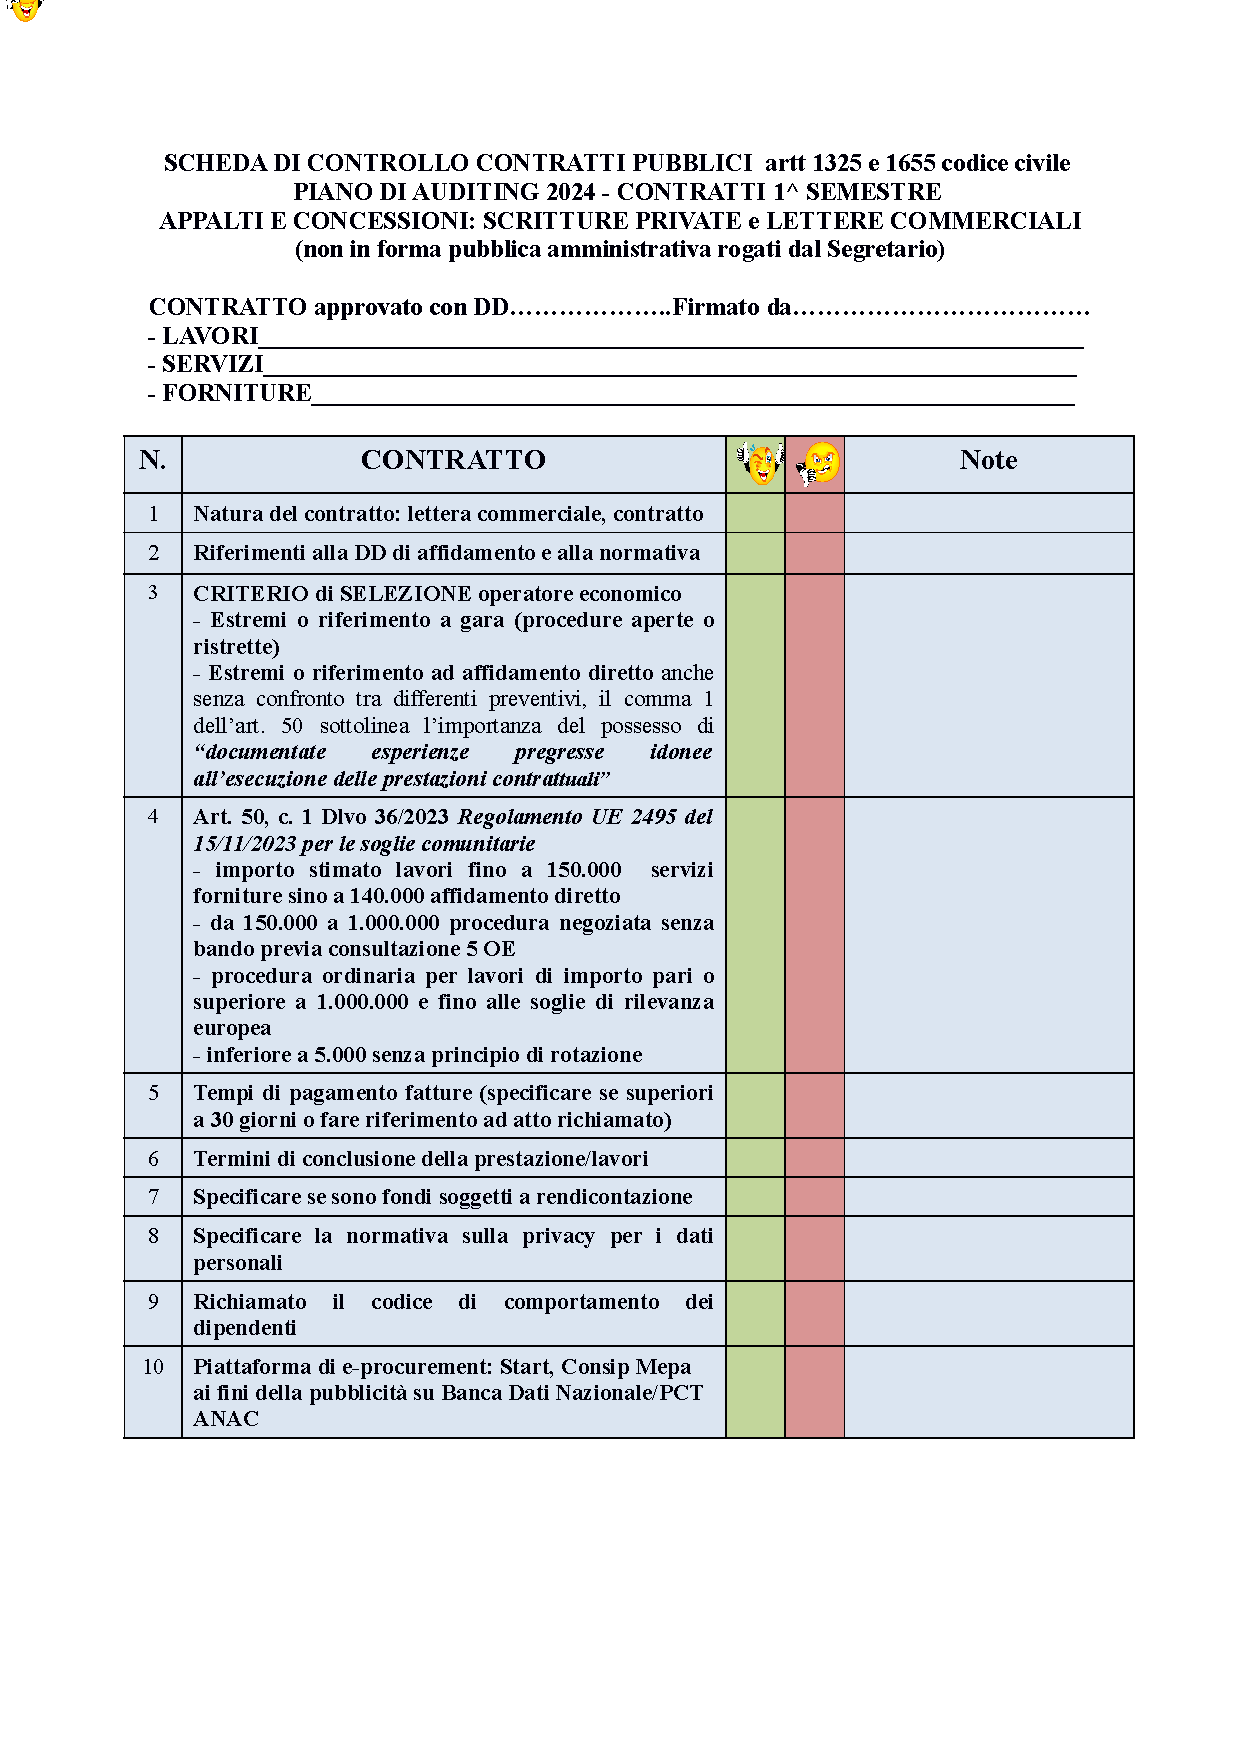
\includepdf[pages=-,scale=0.95,pagecommand={\section*{}}]{Checklists/Lucca/Contratti}
 
\end{document}